\documentclass[11pt,a4paper]{article}
\usepackage[a4paper,top=22mm,bottom=24mm,left=25mm,right=25mm,headheight=15pt,headsep=7mm,footskip=12mm]{geometry}
\usepackage{fontspec}
\usepackage{amsmath,amssymb,mathtools,booktabs,tabularx,array}
\usepackage{xcolor,hyperref,fancyhdr,titlesec,lastpage,orcidlink,tikz,caption}
\usetikzlibrary{arrows.meta,positioning}
\definecolor{ink}{HTML}{111827}
\definecolor{muted}{HTML}{667085}
\definecolor{rulec}{HTML}{D0D5DD}
\definecolor{accent}{HTML}{174EA6}
\definecolor{orcidgreen}{HTML}{A6CE39}
\setmainfont{Norasi.otf}[Ligatures=TeX,BoldFont=Norasi-Bold.otf,ItalicFont=Norasi-Italic.otf,BoldItalicFont=Norasi-BoldItalic.otf]
\newfontfamily\uisans{Garuda.otf}[Ligatures=TeX,BoldFont=Garuda-Bold.otf,ItalicFont=Garuda-Oblique.otf,BoldItalicFont=Garuda-BoldOblique.otf]
\XeTeXlinebreaklocale "th"
\XeTeXlinebreakskip=0pt plus .75pt
\emergencystretch=0.8em
\setlength{\parindent}{1.15em}
\setlength{\parskip}{0pt}
\setlength{\abovedisplayskip}{8pt plus 2pt minus 2pt}
\setlength{\belowdisplayskip}{8pt plus 2pt minus 2pt}
\setlength{\textfloatsep}{12pt plus 2pt minus 2pt}
\setlength{\intextsep}{10pt plus 2pt minus 2pt}
\hypersetup{
  colorlinks=true, linkcolor=ink, citecolor=accent, urlcolor=accent,
  pdftitle={การจัดพิมพ์วิชาการภาษาไทยระดับสากลด้วย LaTeX},
  pdfauthor={Yaoharee Lahtee},
  pdfsubject={Thai academic typesetting and publication workflow},
  pdfkeywords={Thai; XeLaTeX; arXiv; typography; publication}
}
\newcommand{\TB}{\penalty0\hskip0.16em plus0.035em minus0.015em\relax}
\newcommand{\MetaSep}{\hspace{0.6em}\textcolor{rulec}{\textbullet}\hspace{0.6em}}
\titleformat{\section}{\uisans\bfseries\fontsize{12.2}{14.5}\selectfont\color{ink}}{\thesection}{0.55em}{}
\titlespacing*{\section}{0pt}{12pt}{5pt}
\titleformat{\subsection}{\uisans\bfseries\fontsize{10.8}{13}\selectfont\color{ink}}{\thesubsection}{0.5em}{}
\titlespacing*{\subsection}{0pt}{9pt}{4pt}

\fancypagestyle{main}{%
  \fancyhf{}
  \fancyhead[L]{\uisans\fontsize{8.2}{9.5}\selectfont\textcolor{muted}{YAOHAREE LAHTEE}}
  \fancyhead[R]{\uisans\fontsize{8.2}{9.5}\selectfont\textcolor{muted}{THAI ACADEMIC TYPESETTING SYSTEM}}
  \renewcommand{\headrulewidth}{0.35pt}
  \fancyfoot[L]{\uisans\fontsize{7.8}{9}\selectfont\textcolor{muted}{PREPRINT \MetaSep CC BY 4.0}}
  \fancyfoot[C]{\uisans\fontsize{7.8}{9}\selectfont\textcolor{muted}{\thepage\ / \pageref*{LastPage}}}
  \fancyfoot[R]{\uisans\fontsize{7.8}{9}\selectfont\textcolor{muted}{DOI: 10.XXXX/ocsi.2026.001}}
  \renewcommand{\footrulewidth}{0.25pt}
}
\fancypagestyle{first}{%
  \fancyhf{}
  \fancyhead[L]{\uisans\fontsize{8.2}{9.5}\selectfont\textcolor{muted}{OPEN CIVIL SCIENCE INITIATIVE \MetaSep PREPRINT}}
  \fancyhead[R]{\uisans\fontsize{8.2}{9.5}\selectfont\textcolor{muted}{arXiv:XXXX.XXXXX \MetaSep v1.0}}
  \renewcommand{\headrulewidth}{0.35pt}
  \fancyfoot[L]{\uisans\fontsize{7.8}{9}\selectfont\textcolor{muted}{OPEN ACCESS \MetaSep CC BY 4.0}}
  \fancyfoot[C]{\uisans\fontsize{7.8}{9}\selectfont\textcolor{muted}{\thepage\ / \pageref*{LastPage}}}
  \fancyfoot[R]{\uisans\fontsize{7.8}{9}\selectfont\textcolor{muted}{OCSI-TH-2026-001}}
  \renewcommand{\footrulewidth}{0.25pt}
}
\pagestyle{main}

\begin{document}
\thispagestyle{first}
\begin{center}
{\uisans\fontsize{8.2}{10}\selectfont\bfseries\textcolor{accent}{RESEARCH ARTICLE / METHODS PAPER}\par}
\vspace{7pt}
{\uisans\bfseries\fontsize{20.5}{24}\selectfont\color{ink} การจัดพิมพ์วิชาการภาษาไทยระดับสากลด้วย LaTeX:\par
ระบบจังหวะภาษา สมการ ตาราง และการตรวจคุณภาพ PDF\par}
\vspace{9pt}
{\fontsize{10.8}{13}\selectfont\textbf{Yaoharee Lahtee}\,\orcidlink{0009-0005-3861-0626}\par}
{\fontsize{9.5}{11.5}\selectfont Open Civil Science Initiative, Bangkok, Thailand\par}
{\uisans\fontsize{8.4}{10}\selectfont\textcolor{muted}{Corresponding author: [research email] \MetaSep Updated 19 September 2026 \MetaSep Version 1.0}\par}
\end{center}
\vspace{6pt}
\begin{center}
\begin{minipage}{0.90\linewidth}
\noindent\rule{\linewidth}{0.35pt}\par\vspace{5pt}
{\uisans\bfseries\fontsize{9.5}{11}\selectfont บทคัดย่อ}\par\smallskip
{\fontsize{10.1}{13.5}\selectfont\setlength{\emergencystretch}{2em}
ระบบจัดพิมพ์ภาษาไทยระดับสากลต้องรักษาความหมาย\TB จังหวะการอ่าน\TB ความสมบูรณ์ของ Unicode\TB และข้อจำกัดของพื้นที่พิมพ์พร้อมกัน\TB งานนี้เสนอสถาปัตยกรรมการผลิตเอกสารที่ให้ semantic composition มาก่อนการจัดหน้า\TB แล้วใช้ XeLaTeX เป็น compositor พร้อมกฎป้องกันสมการและตารางล้น\TB การฝังฟอนต์\TB metadata\TB และ text layer ของ PDF\TB เป้าหมายไม่ใช่เพียงให้ไฟล์ compile ผ่าน\TB แต่ให้ต้นฉบับอ่านดี\TB ตรวจสอบได้\TB และพร้อมต่อการเผยแพร่แบบ preprint หรือวารสาร}\par
\vspace{5pt}\noindent\rule{\linewidth}{0.35pt}
\end{minipage}
\end{center}
\vspace{5pt}
\noindent{\uisans\fontsize{8.55}{10.3}\selectfont\textbf{คำสำคัญ:} ภาษาไทย; XeLaTeX; arXiv; academic typography; semantic breathing; publication QA}\par
\vspace{7pt}
\noindent{\uisans\fontsize{7.9}{9.6}\selectfont\textcolor{muted}{%
\begin{tabularx}{\linewidth}{@{}>{\bfseries}lX>{\bfseries}lX@{}}
Article ID & OCSI-TH-2026-001 & ORCID & 0009-0005-3861-0626\\
DOI & 10.XXXX/ocsi.2026.001 & Repository & arXiv:XXXX.XXXXX\\
\end{tabularx}}}\par
\vspace{6pt}

\section{บทนำ}
\fontsize{10.6}{14.1}\selectfont
การจัดหน้าเอกสารวิชาการภาษาไทยไม่ควรเริ่มจากการบีบเนื้อหาให้พอดีกับกรอบ\TB แต่ควรเริ่มจากการรักษาหน่วยความหมายและลำดับเหตุผล\TB แล้วจึงเลือกวิธีจัดบรรทัดให้เหมาะกับพื้นที่จริง\TB หลักนี้สำคัญเพราะช่องว่างในภาษาไทยไม่ได้ทำหน้าที่เหมือนภาษาอังกฤษทุกกรณี\TB และการบังคับ justification ที่ผิดวิธีสามารถสร้างช่องไฟขนาดใหญ่จนรบกวนการอ่านได้

ในระบบระดับ production\TB ผู้เขียนควรสามารถเปลี่ยนจากหนึ่งคอลัมน์ไปสองคอลัมน์โดยไม่ต้องเขียนเนื้อหาใหม่\TB ขณะที่สมการ\TB ตาราง\TB รูป\TB การอ้างอิง\TB ORCID\TB DOI\TB และ metadata อื่นยังคงรักษาความสัมพันธ์เดิม\TB ดังนั้นสิ่งที่ต้องออกแบบจึงไม่ใช่แค่หน้าเอกสาร\TB แต่เป็นกฎการตัดสินใจของ compositor ทั้งระบบ

\section{โครงสร้างการจัดพิมพ์}
องค์ประกอบหลักสามารถสรุปเป็นสามชั้น: ชั้นความหมาย\TB ชั้น layout\TB และชั้นตรวจคุณภาพไฟล์สุดท้าย\TB โดยให้คุณภาพรวมเป็นผลคูณของแต่ละชั้น
\begin{equation}
Q_{\mathrm{pub}}
=Q_{\mathrm{semantic}}\,Q_{\mathrm{layout}}\,Q_{\mathrm{PDF}},
\qquad 0\le Q_i\le 1.
\label{eq:qpub}
\end{equation}
หากชั้นใดชั้นหนึ่งล้มเหลว\TB เช่น glyph หายหรือสมการถูกบีบจนอ่านไม่ได้\TB ระบบต้องถือว่าผลลัพธ์ไม่ผ่าน แม้หน้ากระดาษโดยรวมจะดูเรียบร้อยก็ตาม

\begin{center}
\begin{minipage}{0.96\linewidth}
\centering
\captionof{table}{ลำดับการตอบสนองเมื่อองค์ประกอบเสี่ยงล้นพื้นที่พิมพ์}\label{tab:overflow}
\small
\begin{tabularx}{\linewidth}{@{}>{\bfseries}lXl@{}}
\toprule
องค์ประกอบ & การแก้ลำดับแรก & ทางเลือกสุดท้าย\\
\midrule
สมการยาว & split, aligned, multline หรือ full-width & scale แบบมีเกณฑ์\\
ตารางกว้าง & reflow, tabularx, span columns, landscape & scale แบบจำกัด\\
ข้อความไทย & semantic recompose และ line-fit & manual break เฉพาะกรณี\\
\bottomrule
\end{tabularx}
\end{minipage}
\end{center}

\section{จังหวะภาษาและ line fit}
จังหวะที่เป็นธรรมชาติไม่ควรแบ่งเป็นหน่วยเท่ากันตลอด\TB ระบบควรอนุญาตให้หน่วยสั้น\TB กลาง\TB และยาวสลับกันตามน้ำหนักของความคิด\TB จากนั้นจึงค่อยตรวจว่าการรวมหน่วยเหล่านี้ลงหนึ่งบรรทัดก่อให้เกิดช่องไฟผิดปกติหรือไม่\TB หลักนี้ช่วยให้การแก้ layout ไม่ย้อนกลับไปบังคับโครงสร้างภาษา

\section{สมการที่ยาวและการแตกโครงสร้าง}
เมื่อสมการยาวเกินความกว้างของบรรทัด\TB การลดขนาดตัวอักษรไม่ควรเป็นคำตอบแรก\TB ระบบควรแตกโครงสร้างทางคณิตศาสตร์ให้สะท้อนตรรกะของนิพจน์ก่อน เช่น
\begin{equation}
\begin{aligned}
\mathcal{K}_A(W)=1
\quad\Longleftrightarrow\quad
&\sup_{\nu\in\mathcal{V}(W)}
\operatorname{Dist}\!\left(R_A^{\nu}[n],R_A[n]\right)\le\varepsilon_K,\\[-1mm]
&\text{for every admissible variation }\nu\text{ on }W.
\end{aligned}
\label{eq:stable}
\end{equation}
การแบ่งบรรทัดเช่นนี้คงลำดับเหตุผลของสมการไว้\TB และทำให้หมายเลขสมการยังคงอยู่ในตำแหน่งที่ผู้อ่านคาดหมาย

\section{ตารางและความหนาแน่นข้อมูล}
ตารางระดับวารสารควรใช้เส้นแนวนอนเท่าที่จำเป็น\TB หลีกเลี่ยงเส้นกรอบทุกช่อง\TB และจัดคอลัมน์ข้อความให้มีพื้นที่ reflow ก่อนเลือกการย่อทั้งตาราง\TB หากข้อมูลซับซ้อนมากควรแยกเป็นตารางเต็มหน้า\TB landscape\TB หรือภาคผนวกแทน

\section{Publication metadata และความตรวจสอบย้อนกลับ}
ORCID ทำหน้าที่เชื่อม author identity เข้ากับระบบภายนอก\TB ขณะที่ DOI\TB repository identifier\TB article version\TB license\TB และวันที่ปรับปรุงช่วยให้ผู้อ่านระบุฉบับที่กำลังอ้างถึงได้ถูกต้อง\TB metadata เหล่านี้ควรปรากฏทั้งในหน้ากระดาษและใน PDF metadata โดยไม่แย่งลำดับสายตาจากชื่อบทความและบทคัดย่อ

\begin{center}
\centering
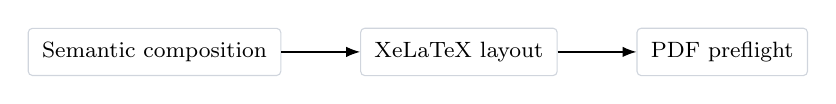
\begin{tikzpicture}[node distance=10mm,>=Latex, every node/.style={font=\uisans\fontsize{8.5}{10}\selectfont}]
\node[draw=rulec,rounded corners=1.5pt,inner sep=5pt] (sem) {Semantic composition};
\node[draw=rulec,rounded corners=1.5pt,inner sep=5pt,right=of sem] (tex) {XeLaTeX layout};
\node[draw=rulec,rounded corners=1.5pt,inner sep=5pt,right=of tex] (qa) {PDF preflight};
\draw[->,line width=.45pt] (sem) -- (tex);
\draw[->,line width=.45pt] (tex) -- (qa);
\end{tikzpicture}
\captionof{figure}{Publication pipeline ที่แยกความหมายออกจาก compositor และการตรวจไฟล์สุดท้าย}
\label{fig:pipeline}
\end{center}

\section{เกณฑ์ยอมรับ}
ต้นฉบับถือว่าผ่านเมื่อไม่มีข้อความหรือวัตถุหลุดขอบ\TB ไม่มี missing glyph\TB ฟอนต์ถูกฝัง\TB ToUnicode map ใช้งานได้\TB การคัดลอกภาษาไทยไม่เสียลำดับอักขระ\TB reference และ citation resolve ครบ\TB และทุกหน้าผ่าน visual review\TB เกณฑ์เหล่านี้เปลี่ยนการจัดหน้าให้เป็นกระบวนการตรวจสอบที่ทำซ้ำได้ มากกว่าการพึ่งความรู้สึกว่าหน้าเอกสาร “ดูดีพอ”

\vfill
\noindent\rule{\linewidth}{0.35pt}\par
{\uisans\fontsize{7.8}{9.4}\selectfont\textcolor{muted}{\textbf{Citation draft:} Lahtee, Y. (2026). การจัดพิมพ์วิชาการภาษาไทยระดับสากลด้วย LaTeX. Open Civil Science Initiative. Preprint.}}
\end{document}
